\documentclass[11pt]{article}
\usepackage[margin=1in]{geometry}
\usepackage{amsmath, amssymb, amsthm}
\usepackage{mathtools}
\usepackage{hyperref}
\usepackage{xcolor}
\usepackage{tikz}
\usepackage{microtype}
\usepackage{parskip}
\usepackage{enumitem}

\hypersetup{
  colorlinks=true,
  urlcolor=blue!55!black,
  linkcolor=black,
  citecolor=black,
}

\title{The Galton--Watson Branching Process\\[2pt]
  \large A note on the extinction fixed point}
\author{Giulio \& Klaus}
\date{Math Corner --- May 2026}

\newtheorem{theorem}{Theorem}
\newtheorem{lemma}[theorem]{Lemma}
\newtheorem{proposition}[theorem]{Proposition}

\begin{document}
\maketitle

\section*{A short note}
\noindent Dear reader,

\smallskip
\noindent This little note accompanies the interactive demo at
\texttt{galton\_watson.html} and walks through the elegant piece of
mathematics behind it: why the extinction probability of a branching
process is the smallest fixed point of the offspring generating
function in $[0,1]$. We tried to keep the prose conversational; the
mathematics is what it is. There are several closely related objects
in play --- an offspring random variable, a population sequence, two
families of generating functions --- and it is easy to get lost in
indices, so $\S 2$ pins the notation down once and for all.

\smallskip
\hfill --- Giulio \& Klaus

\section{Setup}
Let $X$ be a random variable taking values in $\mathbb{N}_0 = \{0, 1, 2, \dots\}$, with distribution
\[
p_k \;:=\; \mathbb{P}(X = k), \qquad k \in \mathbb{N}_0, \qquad \sum_{k \geq 0} p_k = 1.
\]
We call $X$ the \emph{offspring random variable} and $(p_k)_{k \geq 0}$ the \emph{offspring distribution}. To avoid trivialities we assume $p_1 \neq 1$ throughout (no purely deterministic process).

Now build the process. For every $n \geq 1$ and every $i \geq 1$, let
\[
X_{n,i} \quad\text{be an independent copy of } X,
\]
all jointly independent. Think of $X_{n,i}$ as the offspring count of the $i$-th individual in generation $n-1$ (so $X_{n,i}$ contributes to generation $n$). The population sequence is defined by $Z_0 = 1$ and
\[
Z_n \;:=\; \sum_{i = 1}^{Z_{n-1}} X_{n, i}, \qquad n \geq 1,
\]
where the empty sum is $0$ (a dead lineage stays dead). The sequence $(Z_n)_{n \geq 0}$ is the \emph{Galton--Watson process}.

The basic --- and also the most romantic --- question is:
\begin{center}
  \emph{What is the probability $q$ that the lineage ever dies out?}
\end{center}
\[
q \;:=\; \mathbb{P}\!\left(\,\exists\, n \in \mathbb{N} : Z_n = 0\,\right).
\]

\section{Notation, pinned down}
We are about to juggle two generating functions and a few sequences. Let us name them once and never mix them up again:

\begin{center}
\renewcommand{\arraystretch}{1.35}
\begin{tabular}{@{}l@{\quad}l@{}}
\hline
\textbf{Symbol} & \textbf{Definition} \\
\hline
$X$           & the offspring random variable, $X \sim (p_k)$ \\
$\mu$         & mean number of offspring, $\mu := \mathbb{E}[X]$ \\
$Z_n$         & population at generation $n$. $Z_0 = 1$ \\
$f(s)$        & pgf of a single offspring: $f(s) := \mathbb{E}\!\left[s^X\right] = \sum_{k \geq 0} p_k s^k$ \\
$f_n(s)$      & pgf of generation $n$: $f_n(s) := \mathbb{E}\!\left[s^{Z_n}\right]$ \\
$q_n$         & probability of extinction by time $n$: $q_n := \mathbb{P}(Z_n = 0) = f_n(0)$ \\
$q$           & total extinction probability: $q := \lim_{n \to \infty} q_n$ \\
\hline
\end{tabular}
\end{center}

A few comments to keep things from drifting:
\begin{itemize}[leftmargin=*, itemsep=2pt]
  \item $f$ is the pgf of \emph{one} individual's offspring count. It does not depend on $n$.
  \item $f_n$ is the pgf of \emph{the whole population} at generation $n$. It does depend on $n$.
  \item In particular $f_0(s) = \mathbb{E}[s^{Z_0}] = \mathbb{E}[s^1] = s$ (the identity), and $f_1(s) = \mathbb{E}[s^X] = f(s)$.
  \item We will prove that $f_n = \underbrace{f \circ f \circ \cdots \circ f}_{n \text{ copies}}$ --- this is the whole structural content of the process.
\end{itemize}

Throughout, $s$ is a dummy variable in $[0, 1]$. We never differentiate at $s > 1$; everything we need lives on the unit interval.

\section{Three structural facts about \texorpdfstring{$f$}{f}}
Before we touch the recursion, note three properties of the offspring pgf $f$ on $[0,1]$ that we will lean on repeatedly:

\begin{enumerate}[label=(\arabic*), leftmargin=*, itemsep=2pt]
  \item $f(0) = p_0$ and $f(1) = \sum_k p_k = 1$.
  \item $f$ is non-decreasing on $[0,1]$: differentiating term by term, $f'(s) = \sum_{k \geq 1} k p_k s^{k-1} \geq 0$.
  \item $f$ is convex on $[0,1]$: $f''(s) = \sum_{k \geq 2} k(k-1) p_k s^{k-2} \geq 0$.
\end{enumerate}
The mean offspring count is
\[
\mu \;=\; \mathbb{E}[X] \;=\; f'(1) \;=\; \sum_{k \geq 1} k p_k.
\]
This single number controls everything that follows.

\section{The recursion: \texorpdfstring{$f_n = f^{\circ n}$}{fn = f circ n}}
Here is the move that turns a hard probability question into a fixed-point problem in one dimension.

\begin{lemma}[Iteration of the pgf]\label{lem:iter}
For all $n \geq 0$ and all $s \in [0, 1]$:
\[
f_{n+1}(s) \;=\; f_n\!\left(f(s)\right) \;=\; f\!\left(f_n(s)\right).
\]
Consequently $f_n = \underbrace{f \circ f \circ \cdots \circ f}_{n \text{ times}}$, with the convention $f_0 = \mathrm{id}$.
\end{lemma}

\begin{proof}
We prove the first equality, $f_{n+1}(s) = f_n(f(s))$. Recall
\[
Z_{n+1} \;=\; \sum_{i=1}^{Z_n} X_{n+1, i},
\]
where the $X_{n+1, i}$ are iid copies of $X$, independent of $Z_n$. Condition on $Z_n$:
\[
\mathbb{E}\!\left[\,s^{Z_{n+1}}\,\big|\,Z_n\,\right]
\;=\; \mathbb{E}\!\left[\,s^{X_{n+1,1} + \cdots + X_{n+1, Z_n}}\,\big|\,Z_n\,\right]
\;=\; \Bigl(\mathbb{E}\!\left[s^X\right]\Bigr)^{\!Z_n}
\;=\; f(s)^{Z_n}.
\]
Now take expectations:
\[
f_{n+1}(s) \;=\; \mathbb{E}\!\left[s^{Z_{n+1}}\right]
           \;=\; \mathbb{E}\!\left[f(s)^{Z_n}\right]
           \;=\; f_n\!\bigl(f(s)\bigr),
\]
where the last equality is just the definition $f_n(t) = \mathbb{E}[t^{Z_n}]$ applied at $t = f(s)$.

The second equality, $f_{n+1}(s) = f(f_n(s))$, comes from a different (and equally valid) decomposition of the same tree: split it after the very first generation. The $Z_1$ children of the root each found their own independent Galton--Watson sub-tree of depth $n$. Writing $W^{(1)}_n, \dots, W^{(Z_1)}_n$ for those sub-trees' generation-$n$ populations,
\[
Z_{n+1} \;=\; W^{(1)}_n + W^{(2)}_n + \cdots + W^{(Z_1)}_n.
\]
The $W^{(j)}_n$ are iid copies of $Z_n$, independent of $Z_1$, each with pgf $f_n$. So conditioning on $Z_1$ and repeating the calculation above with $f_n$ in place of $f$ and $Z_1$ in place of $Z_n$,
\[
f_{n+1}(s) \;=\; \mathbb{E}\!\left[f_n(s)^{Z_1}\right] \;=\; f_1\!\bigl(f_n(s)\bigr) \;=\; f\!\bigl(f_n(s)\bigr).
\]
Finally, since $f_1 = f$, induction on $n$ gives $f_n = f^{\circ n}$.
\end{proof}

This is striking: the entire infinite-dimensional probabilistic apparatus of the branching process is recorded by iterating a single one-dimensional function.

\section{Extinction as a fixed point}
Set $q_n := \mathbb{P}(Z_n = 0) = f_n(0)$. Plug $s = 0$ into Lemma \ref{lem:iter}:
\[
q_{n+1} \;=\; f_{n+1}(0) \;=\; f\!\bigl(f_n(0)\bigr) \;=\; f(q_n).
\]
So the sequence of cumulative extinction probabilities is obtained by iterating $f$ starting from $0$. Because $\{Z_n = 0\} \subseteq \{Z_{n+1} = 0\}$ (extinction is forever), the sequence $(q_n)$ is non-decreasing in $n$ and bounded above by $1$, hence convergent. Its limit equals the probability of \emph{eventual} extinction:
\[
q \;:=\; \lim_{n \to \infty} q_n \;=\; \mathbb{P}\!\left(\bigcup_{n \geq 0} \{Z_n = 0\}\right) \;=\; \mathbb{P}(\text{extinction}).
\]
Letting $n \to \infty$ in $q_{n+1} = f(q_n)$ and using continuity of $f$ on $[0,1]$:
\[
\boxed{\, f(q) \;=\; q. \,}
\]
Conclusion: \emph{$q$ is a fixed point of $f$ in $[0, 1]$}.

\section{Which fixed point?}
Note that $s = 1$ is \emph{always} a fixed point of $f$ on $[0,1]$, since $f(1) = 1$. So just saying $f(q) = q$ does not yet pin $q$ down. The theorem that does:

\begin{theorem}[Extinction theorem]\label{thm:ext}
The extinction probability $q$ is the \emph{smallest} fixed point of $f$ in $[0, 1]$. Equivalently:
\begin{itemize}[leftmargin=*, itemsep=2pt]
  \item if $\mu \leq 1$, then $q = 1$ (extinction is almost certain);
  \item if $\mu > 1$, then $f$ has a unique fixed point $q \in [0, 1)$, and the extinction probability equals it.
\end{itemize}
\end{theorem}

\subsection*{Why \emph{smallest}}
Let $q^\star \in [0,1]$ be any fixed point of $f$. Since $f$ is non-decreasing,
\[
q_0 = 0 \;\leq\; q^\star \;\;\Longrightarrow\;\; q_1 = f(0) \;\leq\; f(q^\star) = q^\star,
\]
and by induction $q_n \leq q^\star$ for every $n \geq 0$. Letting $n \to \infty$: $q \leq q^\star$. So $q$ sits below every fixed point of $f$ in $[0,1]$; it is the smallest.

\subsection*{The geometric heart: a picture}
Theorem \ref{thm:ext} is really a picture. On $[0,1]$ the graph of $f$:
\begin{itemize}[leftmargin=*, itemsep=2pt]
  \item starts at $(0, p_0)$, on or above the horizontal axis;
  \item ends at $(1, 1)$, on the diagonal $y = s$;
  \item is convex (curving upward, away from the diagonal);
  \item arrives at the right-hand endpoint with slope $f'(1) = \mu$.
\end{itemize}
A fixed point of $f$ in $[0,1]$ is a place where this graph meets the diagonal. The slope $\mu$ controls whether that meeting can happen anywhere other than at $(1,1)$:

\medskip
\begin{center}
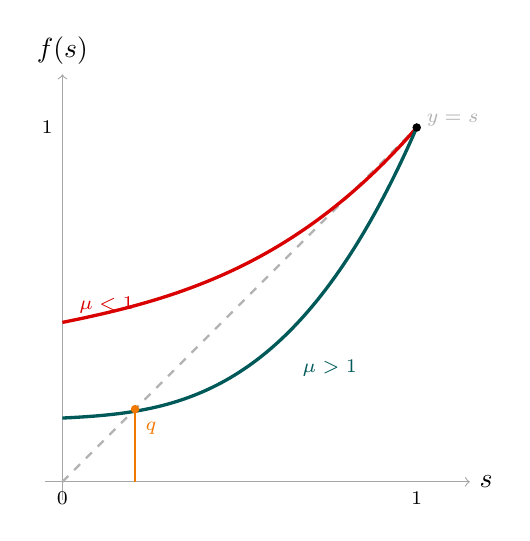
\begin{tikzpicture}[scale=4.5]
  % axes
  \draw[->, gray!70] (-0.05, 0) -- (1.15, 0) node[right, black] {$s$};
  \draw[->, gray!70] (0, -0.05) -- (0, 1.15) node[above, black] {$f(s)$};
  % diagonal
  \draw[gray!60, dashed, thick] (0, 0) -- (1, 1);
  \node[gray!60, right] at (1.0, 1.02) {\scriptsize $y=s$};
  % subcritical curve (mu<1): convex, starting at p0=0.45, ending at (1,1) with slope < 1
  \draw[red!85!black, very thick, smooth, domain=0:1, samples=80]
    plot(\x, {0.45 + 0.20*\x + 0.10*\x*\x + 0.25*\x*\x*\x});
  \node[red!85!black, right] at (0.02, 0.50) {\scriptsize $\mu < 1$};
  % supercritical curve: convex, p0=0.18, slope > 1 at s=1
  \draw[teal!70!black, very thick, smooth, domain=0:1, samples=80]
    plot(\x, {0.18 + 0.05*\x + 0.07*\x*\x + 0.70*\x*\x*\x});
  \node[teal!70!black, right] at (0.65, 0.32) {\scriptsize $\mu > 1$};
  % q for supercritical: crossing near x ~ 0.205
  \fill[orange!95!black] (0.205, 0.205) circle (0.012);
  \draw[orange!95!black, thick] (0.205, 0) -- (0.205, 0.205);
  \node[orange!95!black] at (0.25, 0.15) {\scriptsize $q$};
  \fill[black] (1, 1) circle (0.012);
  \node[below] at (0, 0) {\scriptsize $0$};
  \node[below] at (1, 0) {\scriptsize $1$};
  \node[left] at (0, 1) {\scriptsize $1$};
\end{tikzpicture}
\end{center}

\textbf{Case $\mu \leq 1$.} The curve arrives at $(1,1)$ with slope at most $1$. A convex curve that ends at $(1, 1)$ with slope $\leq 1$ at that endpoint cannot lie below the diagonal anywhere in $[0,1)$ (it would have to curve back upward too steeply at the right endpoint, in contradiction to convexity). So $f(s) > s$ on $[0, 1)$, and the only fixed point in $[0, 1]$ is $s = 1$. Hence $q = 1$.

\smallskip
\textbf{Case $\mu > 1$.} The curve arrives at $(1, 1)$ with slope strictly greater than $1$, so just to the left of $s = 1$ it lies \emph{below} the diagonal. At $s = 0$ the curve is at height $p_0 \geq 0$, on or above the diagonal $y = 0$. (When $p_0 = 0$ the lineage cannot die in one step from a single individual, and indeed $q = 0$ trivially.) By the intermediate value theorem the curve crosses the diagonal somewhere in $(0, 1)$. Convexity forces this crossing to be unique. The crossing is $q$.

The qualitative story is clean: \emph{the dichotomy at $\mu = 1$ is a statement about the angle at which the curve $f$ enters the corner $(1, 1)$.}

\section{Computing \texorpdfstring{$q$}{q} in practice}
Because $f$ is non-decreasing and the smallest fixed point is reached from below, the simplest reliable recipe is to iterate from zero:
\[
q_0 = 0, \qquad q_{n+1} = f(q_n).
\]
This is the same recursion we derived for $\mathbb{P}(Z_n = 0)$, so each iterate has a physical meaning: $q_n$ is the probability the lineage has died out by generation $n$. The sequence converges to $q$ from below, monotonically, and (in the supercritical case) at geometric rate $\mu$.

In the demo you can watch this convergence empirically: pressing \texttt{$\times 100$ batch} runs a hundred independent simulations and the resulting estimate $\hat q$ slides toward the theoretical $q$ shown as a gold dot on the generating-function plot.

\section{Why this is delightful}
The Galton--Watson process is one of the cleanest examples in probability of a recurring pattern in mathematics: \emph{a question about an infinite, branching dynamical system collapses to a one-dimensional fixed-point equation}. The whole long-run behaviour of $(Z_n)_{n \geq 0}$ is read off a single picture --- a curve, a diagonal, where they meet.

This pattern reappears across the subject: in percolation, in the giant component of a random graph, in queueing theory, in epidemic models, in evolutionary biology. It is worth holding on to.

\section*{Where to read more}
\begin{itemize}[leftmargin=*, itemsep=2pt]
  \item K.~Athreya \& P.~Ney, \emph{Branching Processes}, Springer 1972.
  \item T.~Harris, \emph{The Theory of Branching Processes}, 1963.
  \item R.~Lyons \& Y.~Peres, \emph{Probability on Trees and Networks}, freely available online --- chapter 5.
  \item D.~Williams, \emph{Probability with Martingales}, \S 0.5 --- the cleanest one-page treatment in print.
\end{itemize}

\vfill
\noindent\rule{\textwidth}{0.3pt}\\
\textit{Companion to the interactive demo \texttt{galton\_watson.html} --- Math Corner.}
\hfill --- Giulio \& Klaus

\end{document}
